
\documentclass{beamer}
\usepackage[latin1]{inputenc}
%\usetheme{Montpellier}
%\usetheme{Boadilla}
%\usecolortheme[RGB={204,51,255}]{structure}
%\usecolortheme[named=purple]{structure}
\usecolortheme[RGB={62,128,62}]{structure}
%\definecolor{reddish}{rgb}{0.3,0.15,0.3}
%\definecolor{light}{rgb}{0.8,0.6,0.8}
%\definecolor{reddish}{rgb}{.5,0.15,0.15}
\definecolor{reddish}{rgb}{0.5,0.3,0.4}
%\definecolor{light}{rgb}{0.8,0.6,0.8}
\definecolor{reddish}{rgb}{.7,0.25,0.25}
\definecolor{greenish}{rgb}{.25,0.7,0.25}
\definecolor{blueish}{rgb}{.25,0.25,0.7}
\definecolor{purple}{rgb}{.5,0.0,0.5}
\usepackage{graphicx}
\usepackage{pstricks}

\newcommand{\btVFill}{\vskip0pt plus 1filll}

\setbeamertemplate{navigation symbols}{}

\newcommand{\crish}{\color{reddish}}
\newcommand{\cbla}{\color{black}}
\newcommand{\cred}{\color{red}}
\newcommand{\cblu}{\color{blue}}
\newcommand{\cgre}{\color{green}}

\newcommand{\sm}{\color{reddish}$}
\newcommand{\fm}{$\color{black}{}}

\newcommand{\letter}[1]{\color{blue}\texttt{#1}\color{black}}
\newcommand{\binary}[1]{\color{red}\texttt{#1}\color{black}}

\usepackage{tikz}
\usetikzlibrary{arrows,decorations.markings,positioning}
\usepackage{epstopdf}
\usetikzlibrary{fit}

\title[Information Theory lecture 7]{Differential entropy: information theory lecture 6}
\author{COMSM0075 Information Processing and Brain}
\institute{\texttt{comsm0075.github.io}}
\date{October 2020}

\begin{document}

\maketitle

\begin{frame}{Differential entropy}
\textbf{Differential entropy} is the name given to Shannon's entropy for continuous probability distributions
\crish
$$
  h(X)=-\int dx p(x)\log_2{p(x)}
  $$ \cbla
  \end{frame}

\begin{frame}{Example - uniform}
  Consider a uniform distribution
  \crish
  $$
  p(x)=\left\{\begin{array}{ll}1/a&x\in [0,a]\\0&\mbox{otherwise}\end{array}\right.
  $$
  \cbla
  \begin{center}
    \begin{tikzpicture}
    \node[](left){$\ldots$};
    \node[right =  1cm of left](zero){};
    \node[above = 2cm of zero](overzero){};
    \node[right = 0.5cm of overzero](overa){};
    \node[below = 2cm of overa](a){};
    \node[right = 1cm of a](right){$\ldots$};
    \draw[thick] (left) -- (zero.center) -- (overzero.center) -- (overa.center) -- (a.center) -- (right);
    \draw[dotted] (zero.center) -- (a.center);
    \node[below = 0.05 cm of zero](belowzero){$0$};
    \node[below = 0.125 cm of a](belowa){$a$};
    \node[left = 0.0675 cm of overzero](leftoverzero){$1/a$};
    \end{tikzpicture}
  \end{center}
  \end{frame}


\begin{frame}{Example - uniform}
  Consider a uniform distribution
  \crish
  $$
  p(x)=\left\{\begin{array}{ll}1/a&x\in [0,a]\\0&\mbox{otherwise}\end{array}\right.
  $$
  \cbla{}so\crish{}
  $$
  h(X)=-\int_{-\infty}^{\infty}dx\, p(x)\log_2{p(x)}=-\int_0^adx\, \log_2{\frac{1}{a}}
  $$
  \cbla{}
  and so
  \crish
  $$
  h(X)=\log_2{a}
  $$
  \cbla
  \end{frame}


\begin{frame}{Who ordered that!}

  \crish
  $$
  h(X)=\log_2{a}
  $$
  \cbla
  \begin{center}
    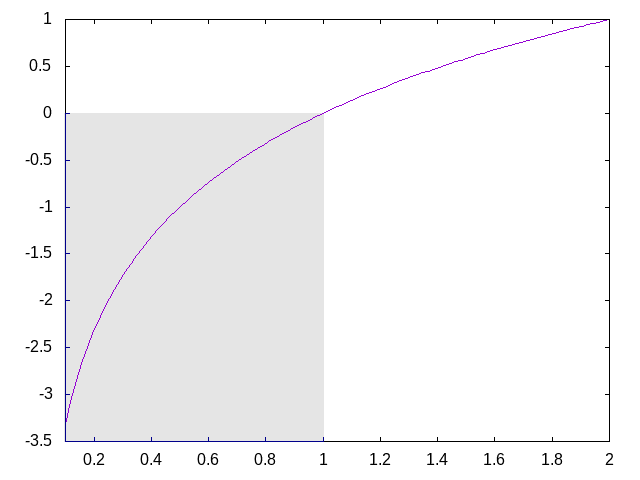
\includegraphics[width=6cm]{log_negative.png}
    \end{center}

\end{frame}

\begin{frame}{Densities are not probabilities}
  \cred
  discrete case $p(x)$ is the probability of $X=x$\\
  \cblu
  continuous case
  $$\int_{x_0}^{x_1}dx p(x)$$ is the probability $x_0\le x< x_1$.
\end{frame}

\begin{frame}{Real numbers are like an infinity of numbers}
  \crish
  1.61803398874989484820458683436563811772030917980576286213544
  8622705260462818902449707207204189391137484754088075386891752
  1266338622235369317931800607667263544333890865959395829056383
  2266131992829026788067520876689250171169620703222104321626954
  8626296313614438149758701220340805887954454749246185695364864
  4492410443207713449470495658467885098743394422125448770664780
  9158846074998871240076521705751797883416625624940758906970400
  0281210427621771117778053153171410117046665991466979873176135
  6006708748071013179523689427521948435305678300228785699782977
  8347845878228911097625003026961561700250464338243776486102838
  3126833037242926752631165339247316711121158818638513316203840
  0522216579128667529465490681131715993432359734949850904094762
  1322298101726107059611645629909816290555208524790352406020172
  7997471753427775927786256194320827505131218156285512224809394
  7123414517022373580577278616008688382952304592647878017889921
  990270776903895$\ldots$
  \end{frame}


\end{document}

